\begin{comment}
							

\end{comment}

\section*{Abstract}
Predicting the next item of a sequence over a finite alphabet has important applications in various domains. \emph{Lossless} approach is a new approach  recently introduced by \citeauthor{gueniche_fournier-viger_tseng_2013} \citeyear{gueniche_fournier-viger_tseng_2013} with CPT. CPT (Compact Prediction Tree) keeps all the training data in order for all the relevant information to be available for each prediction and yield more accurate predictions. Later, CPT+ \cite{gueniche_fournier-viger_raman_tseng_2015} stood as an improved version over CPT. CPT+ improved the high space and time complexity of CPT and increased its accuracy. Compared to other state-of-the-art models from the literature: TDAG, PPM, Lz78, DG, PPM, All-K-order, CPT, CPT+ has the best overall accuracy under evaluation on real life datasets. Recently, CPT+ was used in SPiCe \cite{balle:hal-01399429} competition where it ranked among the best 10 accurate predictors. The competition used a different way of evaluating the predictors from the way that CPT/+ originally evaluated. Hence, its accuracy success is not based on only one particular evaluation, highlighting its importance. 
\par However, even the improved CPT+ utilises a fairly big amount of memory in order to losslessly keep all the training data. This puts some constrains on the size of the training data which will fed CPT+. Tested under real life datasets, CPT+ utilises space from 15 to 175 times more than a \emph{compact representation} of training data. Below, it is presented a \emph{succinct} representation of CPT+ (sCPT) where it consistently utilises from 1.2 to 3 \todo{write theoretic upper bound for sCPT memory usage} times the compact representation of training data, without any significant performance loss in regards to speed. Therefore, sCPT is able to hold undoubtedly more training data, leading to an improved accuracy.


\section{Introduction}
Let a finite set of items (symbols) \(\Sigma = \{e_1, e_2,\ldots,e_\sigma\}\) be called \emph{alphabet}, then a \emph{sequence} \(S\) is a list of ordered items \(S=\langle i_1,i_2,\ldots,i_k\rangle\) where \(i_m \in \Sigma\ for\ 1\leq m \leq k\). A multiset of sequences \(D = \langle S_1, S_2,\ldots,S_l\rangle\) also called \emph{dataset} is constituted by sequences that created under a similar way. Given a dataset, a prediction algorithm is \emph{trained} on this dataset.  Once the prediction algorithm is trained, it will repeatedly accept a \emph{context} which is another sequence of symbols, and outputs a \emph{prediction}. The context is obtained from an unknown \emph{query sequence} which does not belong to the dataset but shares common characteristics with the dataset.  Loosely speaking, the context is derived from a part of the query sequence, and the prediction is about what comes \emph{after} the context in the query. Evaluating the prediction result can be based on different tasks (Appendix \ref{App:predtask}) Each task can be correlated with numerous applications such as, products recommentadionts, web page prefetching, compression algorithms etc. As noted, once the predictor is trained, we are given an unknown query sequence \(Q = \langle q_1, \ldots, q_j, \ldots \rangle\).  The prediction algorithm is given a context \(\langle q_1, q_2,\ldots, q_j,\rangle\) and the predictor aims to say something about what is in \(\langle q_{j+1},q_{j+2},\ldots\rangle\), as it gets explained in Appendix \ref{App:predtask}.

\subsection*{Compact Representation of Training Data}
Compact Representation of training data (\(\Gamma\)) will play an important role as a comparison measure of memory utilisations, during this report. It captures the total size of training data that is given as an input to a predictor. It is defined as \(\Gamma = \log(\sigma) \cdot k \cdot l \) bits and constitutes a base for comparison among different predictors and their memory utilisations.

\subsection*{Lossless}\label{losslessVSlossy}\todo[color=green]{section to be removed; written only for coherence for 2nd year report submission}
Lossless sequence prediction is a relatively new approach and therefore appears to have quite a few challenges that someone that studies it has to cope with. It is clear that due to the fact that a whole dataset is utilised, a lossless approach achieves a higher space utilisation over a lossy approach. This fact leads to two results; firstly, it is somewhat intensive for an algorithm to go through all the data and extract the appropriate information needed for predictions, and secondly, keeping all the relative data \emph{in memory}, through the corresponding data structures, appears to be a considerably hard challenge because the represented structure's space utilisation often reaches an order of magnitude of the initial gathered data. As a result, a lossless sequence prediction approach needs sophisticated tools to search for patterns and sequences in \emph{Big Data} when simultaneously the aforementioned challenges are coped. CPT/CPT+ is currently the only implementations in lossless sequence prediction. 
\par On contrary, a \emph{lossy} approach can be less memory hungry by representing the given information of a dataset through models (like \emph{dependency graphs}) \cite{Padmanabhan:1996:UPP:235160.235164}. This leads to implementation that sometimes utilises less space and can be potentially faster. However, a lossy approach lacks accuracy especially in hard cases when information in a dataset is not repeating as other parts of informations or a repetition is either generalised or ignored by a model having a partly loss of information that is not reversible. Often such hard cases lead to more complex models that along with Big data is hard to make algorithms that produce predictions with efficiency and performance.

\section{CPT and CPT+}\label{CPT}
During this section we present the structures that CPT predictor uses and what is their theoretic memory complexity. Then, we present what additional structures and what strategies CPT+ uses in order for it to approach less memory utilisation than CPT. The predictor of CPT and CPT+ is presented in Section \ref{predictors}. Lastly, we go through strengths and weaknesses of CPT and CPT+ in Section \ref{strength-weaknesses} along with a memory analysis of CPT+ structures (through experimental results with its implementation)
\subsection{Data structures of CPT}

CPT is constituted by a Trie (\emph{Prediction Tree PT}), an Array of bit-vectors (\emph{Inverted Index II}) and an array of pointers to the last items of sequences inserted to the prediction tree (\emph{Look-up Table LT}). As a lossless approach, CPT utilises the whole dataset provided for building its structures.

\subsubsection*{Inverted Index}
The II plays an important role in finding which sequences should be retrieved from the prediction tree. Every bit-vector of the II corresponds to an alphabet item and matches (with 1/0) whether this alphabet item appears to a sequence or not. Every index of a bit-vector belongs to a sequence with the 0\textsuperscript{th} index to belong to the 1\textsuperscript{st} sequence of the dataset and the last index to the last sequence of the dataset (Figure \ref{fig:CPT-structure}). The main operation that is needed is a bit-wise AND among different bit-vectors of the II. Depending on the query sequence items, different bit-vectors are chosen from the II to apply a logical bitwise-AND operation. The result is a bit-vector which shows which sequences contain all the query items. According to the above description, it is easy for someone to oversee that the size of the II is increasing along with the number of sequences. In a real-life application, it is usually the case that the alphabet size remains relatively stable. However, the dataset size can be increased as time passes. An example can be the fact of users' weblogs for a specific website that uses a predictor like CPT for caching web-pages. The website has a determined number of pages (constitutes the alphabet), however, the order that a user visits the pages and the amount of the pages that the user visits per session varies. Hence, different transactions are being created (constituting the sequences). Since the application lies on a lossless approach, it means that the bit-vectors of the II would take more and more space. The II is undeniably the less scalable structure to the CPT which takes \(\mathcal{O}(\sigma \times l)\) bits of space.

\subsubsection*{Look-Up Table}
The Look-Up Table is the structure that adds the necessary ``glue" between the II and the Prediction Tree (figure \ref{fig:CPT-structure}). After that the II calculates which sequences contain the query items then the LT will simply point out to those sequences in the PT. The LT is an array with pointers to every end of every sequence in the PT. The pointer for the 1\textsuperscript{st} sequence is at the 0\textsuperscript{th} position of the LT, the pointer for the 2\textsuperscript{nd} sequence at the 1\textsuperscript{st} position etc. As the II, the size of the LT depends on the number of the sequences that the CPT is trained on. For every sequence, the LT uses 64 bits. In Section \ref{ccpt} we present a more elegant solution where we can omit LT completely.

\subsubsection*{Prediction Tree}
The prediction Tree of the CPT Predictor is constituted by a trie structure (Figure \ref{fig:CPT-structure}). After the build phase where the prediction tree has been built, the main operation that the predictor needs to execute, as a part of a prediction task, is to retrieve back sequences. Which sequences will be retrieved is a matter that is decided by the II. Hence, the prediction tree is important to support instructions that give back the relative sequences. Since the LT points to the end of every sequence, it makes sense to retrieve sequences beginning from root and going up till the root. The retrieved sequence can be reversed in a later time. Therefore, a \emph{getparent()} instruction should be supported in a node of the prediction tree. Currently, the trie offers such functionality which takes \(\mathcal{O}(k)\) time for the sequence retrieval to get completed. The space required for the PT is a factor of the total number of nodes. Every node needs 32 bytes of stored information which includes a pointer to the parent node, pointers to all children nodes and the label of the node.

\begin{figure}[h]
    \centering
    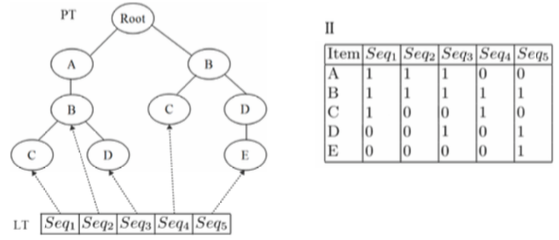
\includegraphics[width=0.75\textwidth]{CPT-structure}
    \caption{A Prediction Tree (PT), Inverted Index (II) and Lookup Table (LT)}
    \label{fig:CPT-structure}
\end{figure}

In Figure \ref{fig:CPT-structure} it is shown an example of CPT during multiple sequence insertions.

\subsection{Data structures of CPT+}
CPT+ keeps the data structure of CPT, however it applies two main new strategies for improving the memory utilisation of CPT \cite{gueniche_fournier-viger_raman_tseng_2015} (Figure \ref{fig:CPTPlus}). The first one, called \emph{Frequent Subsequence Compression (FSC)}, identifies the frequencies of subsequences that appear within a dataset. Each frequent subsequence can be assigned a unique id. This unique id can replace consecutive nodes of the PT that constitute the same subsequence. Of course, a new structure has to be introduced in order to hold the correlation between a frequent subsequence and an id. A \emph{subsequence Dictionary} takes this role and translates a subsequence to an id (or vice-versa) in \(\mathcal{O}(1)\) time. 
\par The second strategy is the \emph{Simple Branches Compression (SBC)}. A \emph{simple branch} is a branch that leads to a single leaf. As a result, each node of a simple branch has between 0 and 1 children. This strategy identifies the simple branches and replaces them with a single node which represents the whole simple branch.

\begin{figure}[h]
    \centering
    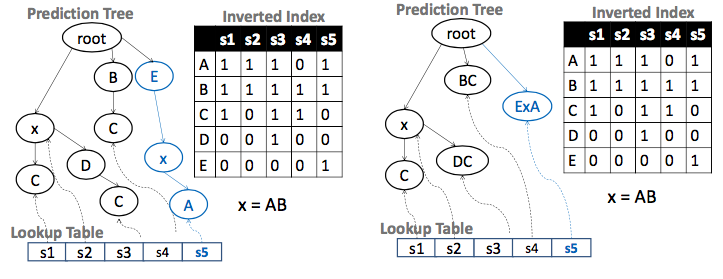
\includegraphics[width=0.80\textwidth]{CPTPlus}
    \caption{FSC and SBC compression strategies}
    \label{fig:CPTPlus}
\end{figure}

\subsection{CPT and CPT+ Predictor}\label{predictors}
In order for the CPT to be used for predictions, the aforementioned data structures have to work together providing the necessary information when it is needed. A bitwise AND shows which sequences contain the query items and then these sequences can be located by using the Look-up Table which points to the end of each corresponding sequence in the PT. Then, PT can be traversed backwards (going to parent until root is reached). Having retrieved a requested sequence from the PT and along with the query sequence, a \emph{consequent} can be resulted as a part of the retrieved sequence. The query items are used as a set of items and each one of these items is matched in the retrieved sequence and removed from it. Having removed all these items from the retrieved sequence, a \emph{consequent} is created. Consequent is eventually the part of the retrieved sequence that specifies what comes next after a query sequence. For example, if the sequence \(S_1=\langle a, b, x, z, c, d, e\rangle\) was retrieved from the prediction tree and the query sequence is \(S_q=\langle a, b, a, c\rangle\) then the consequent will be \(S_c=\langle d, e\rangle\). CPT+ follows the same process for retrieved the matched sequences from PT through LT and II, however as a final step the retrieved sequences has to get \emph{decoded} through the subsequence Dictionary.
\par CPT uses different techniques \cite{gueniche_fournier-viger_tseng_2013} to make use of the consequents. Such techniques could facilitate different prediction tasks (see Appendix \ref{App:predtask}). Recursively shrinking the query size (creating sub-queries) and producing multiple consequents is one of them. All the consequents then are inserted into a table that counts the occurrences of the items. For each consequent a different weight is applied to its occurrences. This weight depends on the length of the corresponding sub-query. Finally, the item with the highest count in the table constitutes the prediction. The process for CPT+ is slightly more efficient since it calculates the sub-queries via a \emph{noise} ratio. This noise ratio is simply a measure to filter the items of the query that have a low frequency in the training data. This low frequency is defined by this ratio. Then, the identified ``noisy" items can be removed one by one, creating the sub-queries and following the same process as CPT.

\subsection{Strengths \& Weaknesses}\label{strength-weaknesses}

CPT and CPT+ (as lossless approaches) utilise all the available sequences in a trie where they are easily accessible through the II and the LT. Therefore, making predictions can be potentially fast and accurate as described in \citep{gueniche_fournier-viger_tseng_2013} and \citep{gueniche_fournier-viger_raman_tseng_2015}. Locating similar sequences can be a relatively easy task that makes CPT and CPT+ work as a good tool for predictors that exploit such sequences. Moreover, CPT can implement all the prediction tasks described in Appendix \ref{App:predtask}, offering a bigger diversity for implementations on several applications. It can be considered undoubtedly as a good state-of-the-art predictor since it is placed among the best 10 best accurate predictors in SPiCe \cite{balle:hal-01399429} competition.
\par \todo{write about training time weakness} 
%Regardless of the space usage limitation that it is already mentioned, there is an extra limitation that can be studied in a near future. That is the fact that the pointers of all the children of a node are being contained in an simple array makes the build phase more and more less efficient for bigger and bigger datasets. That is because for every sequence insertion in the PT, all the children of a node has to be parsed in order to determine whether a new node insertion is required or not. A \emph{Ternary Tree} \cite{bentley_fast_1997} could solve such a problem during the building phase.%
\par However, even though with the improvement of CPT+, where size of the structures were reduced and speed was enhanced, some performance issues can be still addressed. Bit-vectors are the main element of II which is used for locating CPT+'s sequences. When more and more sequences are being added, the bitwise AND operations are becoming slower and slower, leading to performance issues and overall scalability issues since the vectors are becoming much larger. It is common for real life applications to deal with datasets that contain an enormous number of sequences. Therefore, Bit-vectors can be CPT+'s Achilles' heel regarding its performance. Also, space usage of II in such cases can be wasteful since with \emph{Succinct Data Structures} (see Section \ref{App:SDS}) a better and more memory efficient structure can be proposed (section \ref{ccpt}). In addition,  CPT+ suffers from memory consistency making it more hard to predict its behaviour in cases large datasets are fed the predictor, since its overall size depends upon the number of sequences. 
\par It is interesting to point out that one of the two compression strategies of CPT+, partially fails to save space from the PT. The SBC strategy depends on simple branches that lead to a single leaf. However, sequences that share same prefixes will be part of the same single branch. LT will point to all those different sequences that share the same single branch. However, replacing a simple branch with a node will result in conflicts with sequences that share the prefix. LT will still point to nodes that should have been freed. If the memory is indeed freed, then LT points to a ``bad" memory address otherwise memory saved does not correspond to the numbers of nodes replaced during SBC strategy. Looking at Figure \ref{fig:CPTPlus}, let us assume that LT $S_4$ sequence points to x. Thus, $S_4$ is a prefix of $S_5$. If the branch of sequence $S_5$ is identified as a simple branch then node x cannot be freed. LT should still point to x and x would point to node E. In this example, the memory saved is zero. Of course there are workarounds for making SBC strategy work on such cases but it is not studied in \citetitle{gueniche_fournier-viger_raman_tseng_2015}. The memory evaluation made upon the number of nodes saved and not on the actual memory utilisation as reported by the system. Implementation details for CPT and CPT+ can be found on http://goo.gl/LE4uYO.
\par In Figure \ref{fig:CPT_mem} it is presented the memory usage of CPT+ and its data structures as it was reported by Java Virtual Machine (JVM) in respect of each data structure object. For this evaluation, synthetic datasets were used in order to illustrate the linear pattern of the memory increment according to sequence number. Datasets were generated through IBM Quest Dataset Generator \cite{spmf}. It is an interesting fact that CPT+ utilises almost 40 times the space of \(\Gamma\). Even the smallest structure like the LT, is around 5 times of \(\Gamma\). If it is considered that in a lossless approach where all available training data are kept and relatively big quantities of training data might be given, then CPT+ cannot be scalable in applications which depend on \emph{Big Data}. 

\missingfigure{add figure that shows the memory increase for fixed seq count and variable alphabet}

\begin{figure}[h]
    \centering
    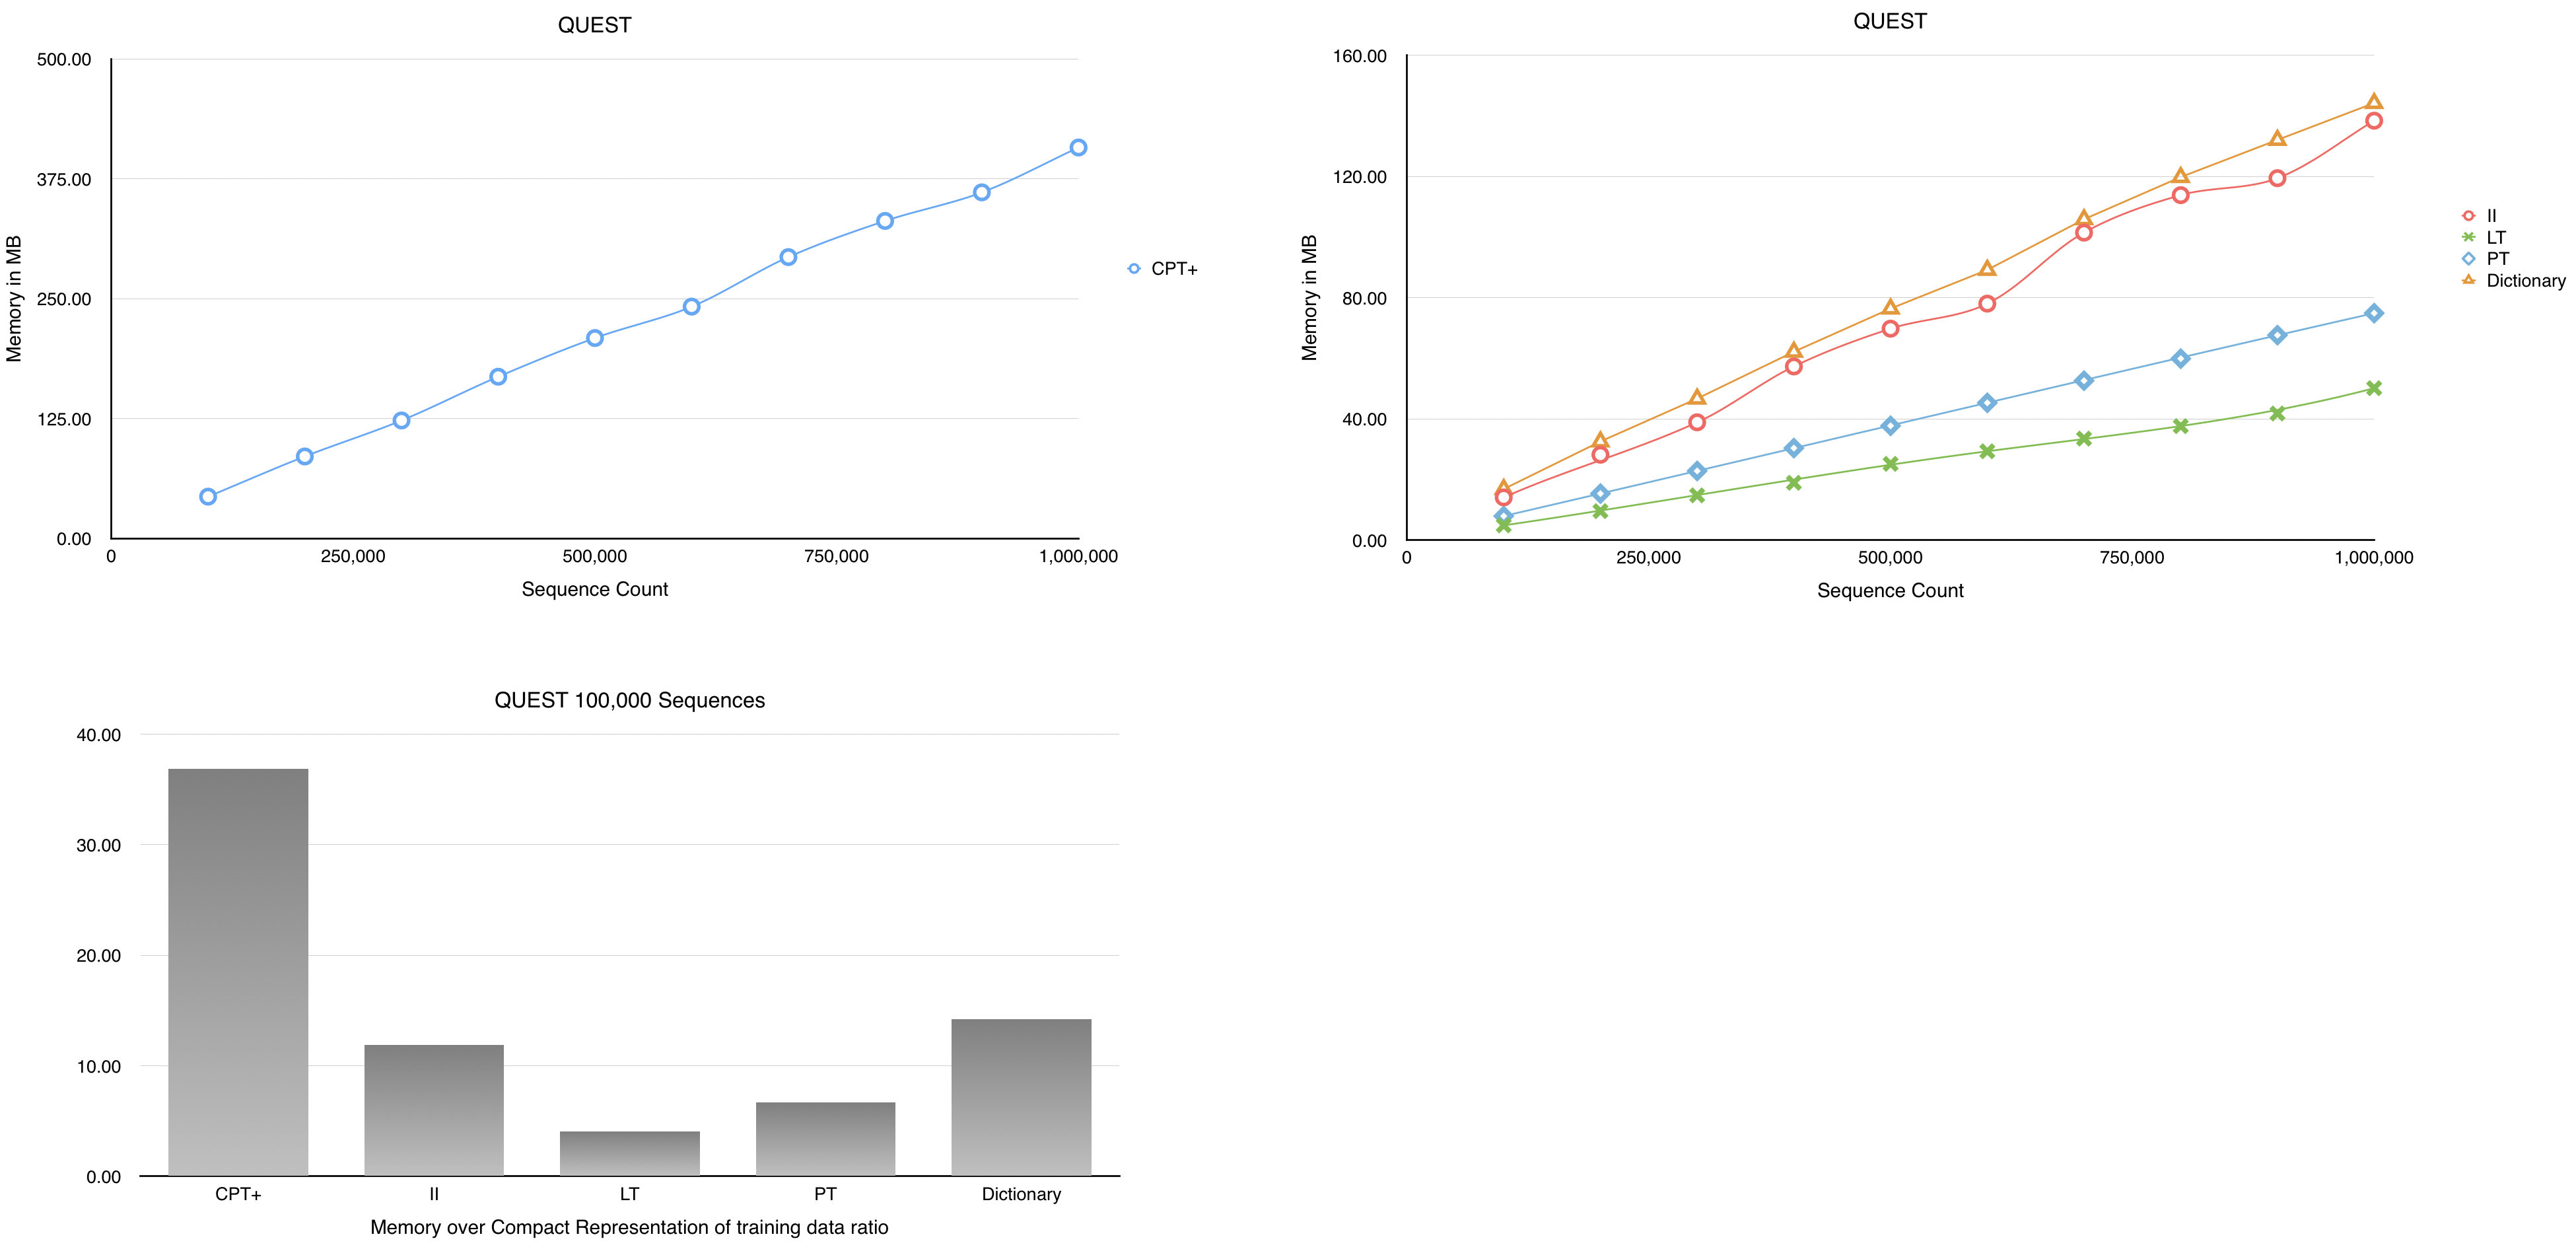
\includegraphics[width=1\textwidth]{CPTPlus_mem}
    \caption{CPT+ memory usage and its structures for datasets of different count number (top); Ratio of CPT+/structures over \(\Gamma\)}
    \label{fig:CPT_mem}
\end{figure}

\section{Succinct CPT}\label{ccpt}
Succinct CPT copes with all the memory disadvantages of CPT by introducing different succinct data structures for the roles of PT, II and LT. By using succinct data structures and fast operations like \emph{rank/select} (Appendix \ref{App:rank_select}), we can achieve a significant memory reduction in performance of CPT+ without relatively sacrificing any speed. The predictor of CPT+ remains the same. This is feasible because the combined succinct data structures offer the same functionalities and instructions as the former CPT+ structures (II, PT, LT). This section will be structured as follows. Firstly,  we present a technique for representing Inverted Indices which takes at most $1\cdot \Gamma$ of space and how this technique can be used for CPT+ predictor functionality. Next, we show how the PT can be represent through a bitmap and how this bitmap can be stored efficiently while it retains the instructions needed for CPT+ predictor. Lastly, we go through the way of omitting the LT structure.
\subsection{Elias-Fano for Inverted indices}\label{elicas_fano}
The II as shown in Figure \ref{fig:CPT-structure} contains which alphabet item is contained in which sequence. However, every bit-vector can be treated as an inverted list of the positions of the set bits. Hence, the bit-vector for item \(A\) of the Figure \ref{fig:CPT-structure} can be written as \(\langle 1, 2, 3\rangle\). Since, every position in the bit-vector is correlated with a sequence serial number (1\textsuperscript{st}, 2\textsuperscript{nd}, \dots, l\textsuperscript{th} sequence) it is obvious to conclude that the aforementioned inverted list is monotone sequence of numbers. This is important because  the compression technique which is mainly being used and described next, is based on \emph{gap encoding}. As it will be proved later, gap encoding will make possible to store the II in space smaller or at least same as the space of the initial dataset. The techniques described below are based on a paper by Elias \cite{elias_efficient_1974} and a paper which demonstrates similar ideas for representing Inverted Indices \cite{vigna_quasi-succinct_2013}.
\subsubsection*{Elias Techinque}
\par It is clear that every bit-vector of the II can be seen as an inverted list of the sequences that the alphabet item is contained. Because the list is monotone can be seen as \[0 \leq x\textsubscript{0} \leq x\textsubscript{1} \leq \dots \leq x\textsubscript{n - 2} \leq x\textsubscript{n - 1} \leq u \] where \(u > 0 \) as a known upper bound. That bound is always known because during prediction phase the dataset size is known too. Now, this list of numbers can be split in two bit arrays according to the formulas below:
	\begin{description}
  	\item[lower bit array:] for every item of the list, the array continuously stores its lower $\lambda$ bits where \(\lambda = max\{0, \lfloor \log(u/n)\rfloor\}\).
  	\item[upper bit array:] then the upper bits are stored in a sequence of unary-coded gaps (see Figure \ref{fig:ef_ex})
	\end{description}

\begin{figure}[h]
    \centering
    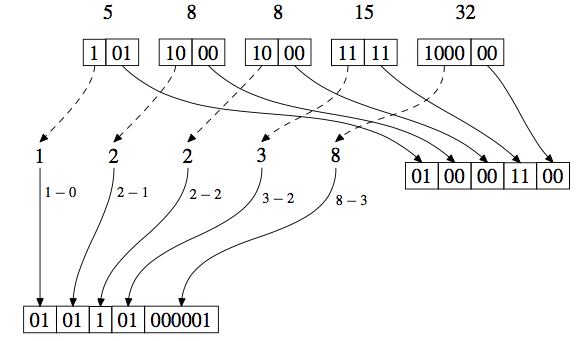
\includegraphics[width=0.75\textwidth]{elias_fano_exmpl}
    \caption{In this example we have a list of numbers 5, 8, 8, 15, 32 with upper bound 36. For the lower bit array \(\lambda = \lfloor \log36/5\rfloor = 2\). On right it is shown all the \(\lambda\) bits of all elements which are gathered together to create the lower-bets array. On left, the gaps for every number upper bits are calculated and stored sequentially in unary code in the upper-bits array.}
    \label{fig:ef_ex}
\end{figure}	
\subsubsection*{Space property}
\par Space wise, it can be proven \cite{vigna_quasi-succinct_2013} that for every item of a list it is used at most \(2 + \lceil\log(u/n)\rceil\) bits. The dataset containing the sequences, from where the II will be created, can be considered as a memoryless source. Then, every symbol appears with a probability of \(p_{\kappa} = \frac{1}{\sigma} \) in the dataset. The bits needed to code a symbol will be \( \sum_{\kappa = 1}^{\sigma} p_{\kappa} \cdot \log(\frac{1}{p_{\kappa}}) = \log(\sigma)\). An II that uses Elias way of recording the set bit positions for every bit-vector, will take a total space:

\begin{equation} \label{II_ef_mem}
\sum_{\iota = 1}^{\sigma} n_{\iota}\cdot ( \log(\frac{l}{n_{\iota}}) + 2 )
\end{equation}

We set as \(M\) to be the total length of the dataset. Then:

\begin{equation} \label{II_dataset}
	M \geq l 
\end{equation} 

Using (\ref{II_ef_mem}), we can oversimplify it as:

\begin{equation}\label{II_em_simplified}
	\sum_{\iota = 1}^{\sigma} n_{\iota}\cdot ( \log(\frac{M}{n_{\iota}}) + 2 )
\end{equation}
For any bit-vector of the II:
\begin{equation} \label{bit_vector_prob}
	p_{\iota} = \frac{n_{\iota}}{M} \textnormal{, using (\ref{II_dataset})}
\end{equation}
Finally, using (\ref{II_em_simplified} and (\ref{bit_vector_prob})), the total memory of an II using Elias technique will be:

\begin{equation} \label{II_ef_mem_final}
	\sum_{\iota = 1}^{\sigma} M\cdot p_{\iota}\cdot ( \log(\frac{1}{p_{\iota}}) + 2 )
\end{equation}

In last equation (\ref{II_ef_mem_final}) and by claiming that the oversimplification at (\ref{II_em_simplified}) is usually \(M > l \), it can be assumed for most cases that the total memory is less than the memory needed to code the whole dataset. So:
\begin{equation}
	\sum_{\iota = 1}^{\sigma} M\cdot p_{\iota}\cdot ( \log(\frac{1}{p_{\iota}})) \leq M\cdot log(\sigma)
\end{equation}
This final statement is important due to the fact that most of the times a usual data structure consumes space that is at least an order of magnitude of the initial input data size. In the above case, the space which is used by an inverted index with Elias Fano representaions, is usually less or the same as the size of the input data.
\subsubsection*{Accessing Values}
\par Accessing and retrieving back any random value \(x_i\) stored with this way can be done  by following the steps on the upper bit array and applying rank/select operations (Appendix \ref{App:rank_select}):
\begin{enumerate}
	\item \(\lbrack \frac{x_i}{2^{\lambda}} \rbrack = \theta \)
	\item \(\varrho = select_0(\theta)\)
	\item \(\zeta = rank_1(\varrho)\)
	\item concatenate (the binary representations) of \(\varrho - \zeta\) with the value of lower bit array at index \(\zeta\)
\end{enumerate}
Similarly, we can continue accessing all the values sequentially by keeping track of the number of the $0_s$ parsed in every position of the upper array. Every time that an $1$ is met then we have met a new stored value and therefore we should concatenate our bits. A $0$ means that we have to increase our variable that counts zeros since the gap to our next number is being increased.
\subsubsection*{II in sCPT}
CPT predictor uses the II in order to determine which sequences contain specific alphabet items. With an II which uses bit-vectors this can be done by applying a bit-wise AND to the relevant bit-vectors. We have studied different ways of representing an II. Such representations were the \emph{Succinct Multibit Tree} (SMBT) \cite{tabei_2012}, the \emph{RRR-vectors} \cite{Raman}, the \emph{Wavelet Tree} (WT) \cite{tabei_tsuda_2011} and the \emph{Word Aligned Hybrid} (WAH) \cite{wu_optimizing_2006}. Elias Fano representation had the best memory performance which can be also proved (see previous section).
\par In inverted indices that follow the Elias gap encoding way, the same functionality can be achieved by \emph{decoding} every list of values for every alphabet item and them by applying an intersection among the relevant lists. However, intersecting lists that might contain a relative big amount of values is inefficient because every intersection will depend on the length of the largest list. With Elias-Fano II we can take advantage of the fact that we can \emph{jump in} a specific value of a list and complete an intersection in relation to the smallest list. Therefore, the overall speed performance is not affected much as shown in experimental evaluation.

\subsection{PT in sCPT}
Currently CPT+ uses trie as a structure in order to store the sequences of a dataset and retrieve the sequences back during prediction phase (Figure \ref{fig:CPT-structure}). However as it has already been mentioned that pointers are needed for every child and parent node in order to represent this linking relation among the nodes. This kind of representation can be a waste of space. On the other hand, having pointers to link nodes together, provide us with a fast, a convenient and a rapid traversal among the trie nodes. Below, it is described a way to reduce the space by a factor of 20 times \todo{put theoretic space (if I can prove it)} and without sacrificing speed performance in terms of the CPT predictor needs.
\subsubsection*{Binary Tree as a Level-order Bitmap}

\begin{figure}
	 \centering
    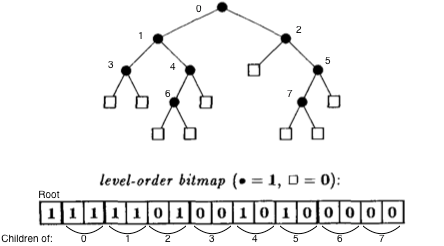
\includegraphics[width=0.75\textwidth]{jacobson_binary_bitmap}
    \caption{Level-order bitmap representation}
    \label{fig:binary_bm}
\end{figure}

A binary tree can be represented as a series of bits, called \emph{bitmap} \cite{jacobson_space-efficient_1989} . Later, it will be shown how relations among nodes can be achieved, same as having a normal binary tree and it can be generalised for any \emph{k-ary} trees. Figure \ref{fig:binary_bm} shows a bitmap representation of a binary tree. In order to produce the bitmap of the binary tree, the tree has to be traversed in level order beginning from the root and writing down the first $1$ of the bitmap. Then, the next level should be traversed where an $1$ is put in the bitmap if there is a node or $0$ in case a node does not exist at the appropriate position. As it can be seen from the figure, the number of $1_s$ written in the bitmap equals to the number of nodes of the binary tree. The overall length of the bitmap is $2 \cdot \eta  + 1$ where $\eta$ is the overall number of nodes of binary tree.
\par Accessing a child or parent node of the tree can now be achieved by applying rank/select operations on the bitmap itself. 
\begin{description}
	\item [get child:] \(rank_1(i) \cdot 2 - 1\)
	\item [get right sibling:] \(rank_1(i) \cdot 2 + 1\)
	\item [get parent:] \(select_1(\frac{i + 1}{2} )\)
\end{description}

Where \(i\) is the index of the node in the bitmap. Looking at Figure \ref{fig:binary_bm}, an example of finding the bitmap index of a parent node located at $9_{th}$ position would be the node located at $4_{th}$ position in the bitmap. That is because the parent node of  node 6 will be the node 4 (counting in level order). Similarly, it can be checked, at any position, whether there is a right sibling or not. If the remaining of the position index divided by 2 is not zero, then there is a right sibling. Accessing a child and getting a sibling is achieved by using rank operation as described.

\subsubsection*{K-ary Trees as Level-order Bitmap}
The binary tree bitmap can easily be generalised to any K-ary tree as shown in Figure \ref{fig:k-ary-bm}. Then accessing child, getting sibling and getting parent are generalised as:

\begin{description}
	\item [get child: ] \(rank_1(i) \cdot K - 1\)
	\item [get right sibling: ] \(rank_1(i) \cdot K + 1\)
	\item [get parent: ] \(select_1(\frac{i + 1}{K} )\)
	\item [sibling exist if: ] remaining of \(\frac{i}{K}\) is not zero
\end{description}

\begin{figure}
	 \centering
    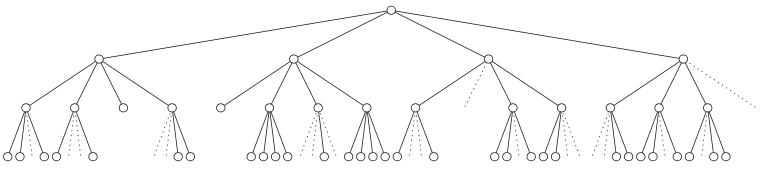
\includegraphics[width=0.75\textwidth]{k-ary_bitmap}
    \caption{Generalized Jacobson encoding of a 4-ary tree: 1111 1111 1111 1011 1110 1101 1001 0000 0011 0000 1111 0010 1111 1001 1101 1100 0011 1101 1011 0000 0000 0000 0000 0000 0000 0000 0000 0000 0000 0000 0000 0000 0000 0000 0000 0000 0000 0000 0000 0000 0000 0000 0000 0000 0000 0000 0000 0000 0000 0000--- 200 bits}
    \label{fig:k-ary-bm}
\end{figure}

\subsubsection*{Storing bitmap}
A relative serious drawback of the described approach for representing a tree using a binary bitmap is the fact that the bitmap gets quite long. The overall length is twice as long as the total number of nodes (for a binary tree). Usually, rank/select operations have a space and time overhead that depends upon the type of the bit-vector that they support. Deciding how to store the bitmap could affect both the memory utilisation and the speed performance. According to SDSL-lite library \cite{gog_2015}, a rank which supports a bit-vector has a 25\% of its total length bits overhead and an \(\mathcal{O}(1)\) time complexity. These stats vary according to the representation of the bit-vector (such other bit-vector representation is RRR-vectors \cite{Raman}). CPT+ predictor is mainly depended on accessing parents nodes since LT points to the end of sequences. Elias Fano representation of bit-vectors, as described in section \ref{elicas_fano}, is implemented with sd-vectors by SDSL-lite library. Getting the parent node in a bitmap requires only select operation. The select operation on a sd-vector has a space overhead of 64 bits and an \(\mathcal{O}(1)\) time complexity. These properties and the way the bitmap is stored (as already explained for inverted indices) make it an ideal option for storing the bitmap of the PT. Accessing the parent node will be achieved quite as fast as in the trie representation of CPT+. At the same time the representation will be succinct which will save a big amount of space. 

\todo[inline]{
Proof that a bitmap stored with Elias Fano will take space up to $\Gamma + 2\cdot M$ 

\[N = \textnormal{ total number of trie nodes}\]
\[M = k \cdot l (\textnormal{ length of the dataset}) \]

The space for the bitmap with Elias Fano is:

\begin{equation} \label{bitmap_mem}
	\begin{gathered}
		N \leq M \\
		\bigg(\log\Big( \frac{(N + 1)\cdot \sigma}{(N + 1)}\Big) + 2\bigg)\cdot N = (\log\sigma + 2)\cdot N = (\log\sigma + 2)\cdot  M = \\
		= \log\sigma\cdot M + 2 \cdot M = \Gamma + 2\cdot M, \textnormal{using definition for } \Gamma
	\end{gathered}
\end{equation}
}
 
\subsection{Look-Up Table Omission}
In CPT+ Look-Up table is used for pointing in the last node of a sequence within the trie. However shown in Figure \ref{fig:LT-ommission}, the nodes of the trie can be counted in a level-order way and thus an II upon the node count would be easy to be constructed. The $1^{st}$ sequence will be the $6_{th}$ column in the inverted index due to the fact that this sequence ends on node 6 in the trie. However, the II length now depends on the total number of trie nodes. The total number of nodes is usually much higher than the total number of sequences (in case that is less due to high sequence repetition then this approach is even better for the II memory utilisation). As a result, the II would contain longer bit-vectors for every alphabet item. It is common to assume that no memory is saved but the opposite happens. On the other hand, sCPT uses bit-vectors coded with Elias Fano technique. It can be proven that the extra overhead per bit-vector will be $log_2(M)$, where $M$ is the ratio of nodes count over sequence number (assuming that node count is higher than sequence number). Also, in most datasets the sequence number is greater than the alphabet size. Thus, this overhead will be less than the 64 bits per sequence which is required by LT. 

\todo[inline]{
In equation (\ref{II_ef_mem_final}), it was proved that an II with Elias Fano represenations takes up to $1\cdot \Gamma$.
However, with the LT omission, we construct II upon the total number of trie nodes ($N$). If $N\leq l$ then (\ref{II_ef_mem_final}) still holds. If $N\geq l$ then the II will take space:
\begin{equation} \label{II_LT_mem}
	\begin{gathered}
		\sum_{\iota = 1}^{\sigma} n_{\iota}\cdot ( \log(\frac{N}{n_{\iota}}) + 2 ), \textnormal{ where: } N = x\cdot l \\
		\Rightarrow \sum_{\iota = 1}^{\sigma} n_{\iota}\cdot ( \log(\frac{x\cdot l}{n_{\iota}}) + 2 ) \\
		\Rightarrow \sum_{\iota = 1}^{\sigma} n_{\iota}\cdot (\log(x) + \log(\frac{l}{n_{\iota}}) + 2 )\\
		\Rightarrow \log(x)\cdot \sum_{\iota = 1}^{\sigma}n_{\iota} + \sum_{\iota = 1}^{\sigma} n_{\iota}\cdot (\log(\frac{l}{n_{\iota}}) + 2 )\\
		\Rightarrow \log(x)\cdot M + \Gamma, \textnormal{using equation (\ref{II_ef_mem_final})} \\
		\Rightarrow \Gamma + \log(\frac{N}{l})\cdot M
	\end{gathered}
\end{equation}

\begin{equation} \label{seq_length}
	\begin{gathered}
		N \leq M \\
		\frac{M}{l} = k, \textnormal{ sequence length}\\
	\end{gathered}
\end{equation}

\par Using  equations (\ref{bitmap_mem}), (\ref{II_LT_mem}) and (\ref{seq_length}), then the total pessimistic memory usage of sCPT will be:

\begin{equation}
	\begin{gathered}
		\Gamma + \log(k)\cdot M + \Gamma + 2\cdot M =\\
		= 2\cdot \Gamma + 2\cdot M + \log(k)\cdot M = \\ = 2\cdot \Gamma + M\cdot (2 + \log(k))
	\end{gathered}
\end{equation}
}

\begin{figure}[h]
    \centering
    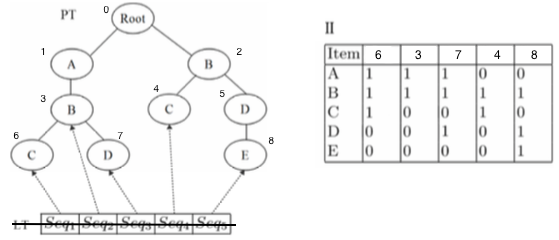
\includegraphics[width=0.75\textwidth]{cpt-lt-ommission}
    \caption{Illustration of how LT can be omitted and have LT take its role}
    \label{fig:LT-ommission}
\end{figure}

\section{Experimental Results and Performance Comparison} \label{experimental}
For the experimental results a C++ version of CPT and CPT+ implemented. The design and architecture is the same as CPT and CPT+ original implementation in Java 8 (provided at http://goo.gl/LE4uYO). The experiments performed on a Intel Xeon CPU E5-2620 v3 at 2.40GHz, Cache 15MB, 16GB Ram DDR4 at 1866MHz. The datasets that were used are available through SPMF library \cite{spmf} and constitute real life datasets. The BMS, Kosarak, MSNBC Fifa, Nasa\_07 and Nasa\_08 datasets consist of webpages logs by users on webpages. SIGN dataset is transcribed from videos, in sign language. BIBLE is constituted by the set of sentences divided into words which represents a sequence. 
\par To evaluate memory, both CPT+ and sCPT were trained with the whole dataset and then the memory calculation performed upon the total memory retained in C++ Heap segment after the training is finished. The speed performance evaluated by feeding the predictor with queries of length 3 items which are generated through the same dataset that trained CPT+ and sCPT respectively. Since the accuracy of the prediction is not currently evaluated and the purpose of this evaluation was to perform a full prediction process (to evaluate speed when predictor does all its steps), a K-Fold \cite{Kohavi} validation environment was not set up. It should pointed out that both CPT+ and sCPT use the exact same predictor. What changes is the instruction call to their data structures respectively.


\subsection*{Space Comparison}
For the space comparisons the compact representation of training data usage ($\Gamma$) will be used as a metric between CPT+ and sCPT. CPT+ utilises $15 \cdot \Gamma$ to $174 \cdot \Gamma$ (Figure \ref{fig:sdvsCPTplus}). sCPT space utilisation lies between $1.2 \cdot \Gamma$ to $4.7 \cdot \Gamma$. The succinct representation of CPT+ can be considered more consistent and predictable since its variance range for memory is much less than CPT+. The inverted indices correspond to the biggest structure in regards of memory consumption among the other structures in CPT+. II in CPT+ takes $0.2 \cdot \Gamma$ to $163 \cdot \Gamma$ while in sCPT $0.5 \cdot \Gamma$ to $2.9 \cdot \Gamma$ (Figure \ref{fig:sdIIvsII}). These comparisons illustrate the memory benefits of sCPT over CPT. Therefore, the ability for sCPT to scale is much greater than this of CPT+.
 \subsection*{Speed Comparison}
Figure \ref{fig:sdvsCPTplus} depicts the speed performance of sCPT opposite to CPT+. Positive number means that sCPT is slower and negative that it is faster. sCPT through experiments found to be 10\% to 60\% slower in half of the datasets while its performance considered the same or slightly faster in the rest of the datasets. The performance differences lie only on the different data structures used in CPT+ and sCPT and not in any variations of the predictor. 
\begin{figure}[h]
    \centering
    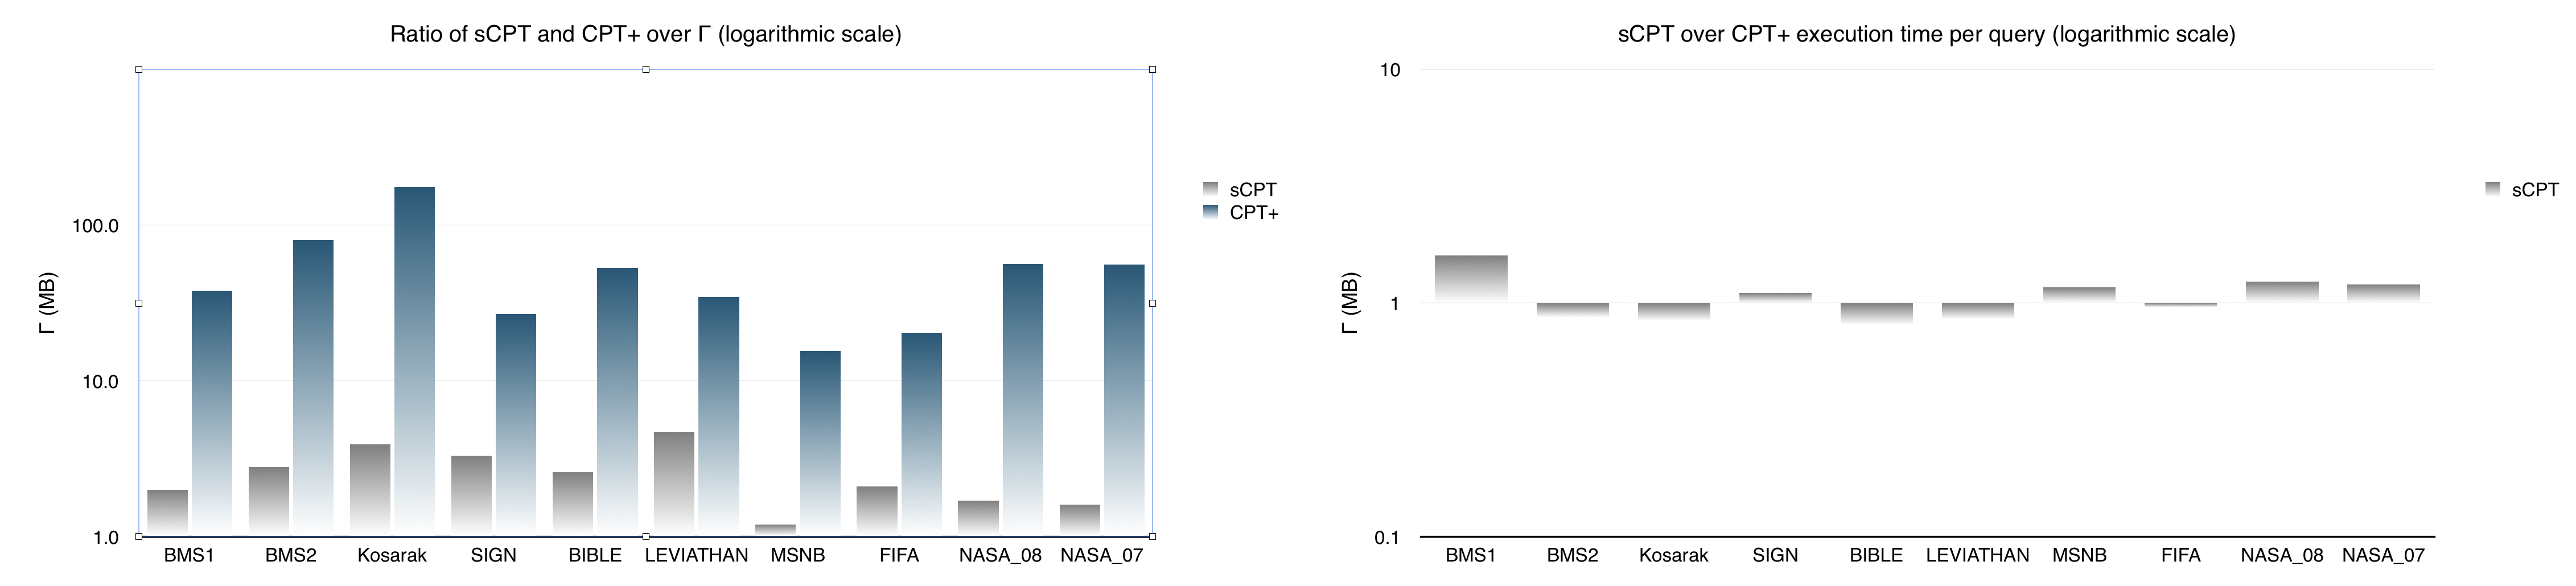
\includegraphics[width=1\textwidth]{sdvsCPTplus}
    \caption{at right: sCPT and CPT+ over $\Gamma$, at left: execution time ratio of sCPT over CPT+. The execution time (clock time) measured for 1000 queries, same for both implementations.}
    \label{fig:sdvsCPTplus}
\end{figure}

\begin{figure}[h]
    \centering
    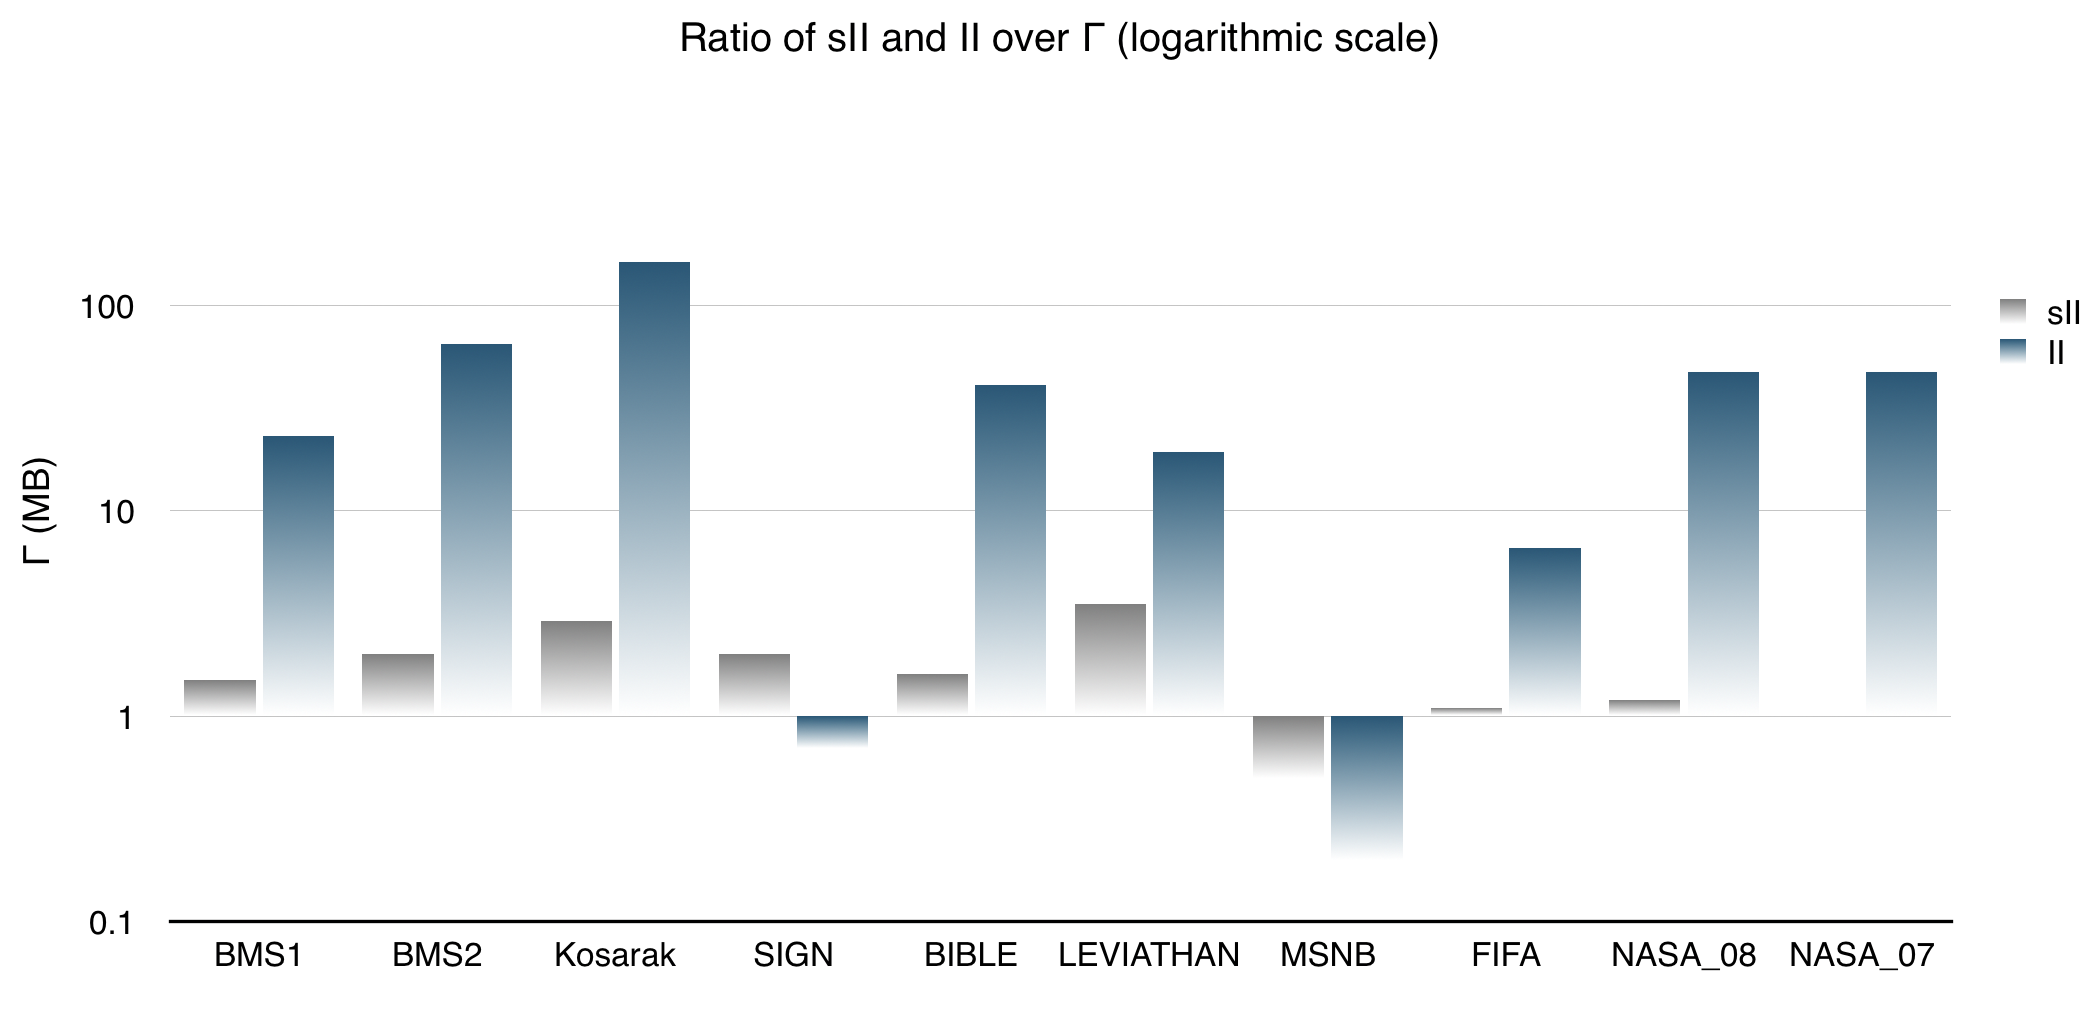
\includegraphics[width=0.75\textwidth]{sdIIvsII}
    \caption{II of sCPT over $\Gamma$ and II of CPT+ over $\Gamma$. Negative number means that the structure takes less space than the compact representation of training data}
    \label{fig:sdIIvsII}
\end{figure}

\section{Conclusion}
CPT+ is proven to be one of the state-of-the-art predictors which ranked among the best in SPiCe competition. However its memory consumption lack of consistency and predictability which make it difficult for CPT+ to scale up as a lossless approach. sCPT overcomes these weaknesses of CPT+ and offers a consistent and predictable memory utilisation without sacrificing any serious amount of performance. With sCPT the ability of greater scalability is offered. As it was already proven by CPT and CPT+, losslessly keeping all the available training data offers greater accuracy. As a future work for sCPT would be to evaluate the fact that scaling the lossless predictor in a factor where much more training data is available, would improve prediction accuracy even more.


\newpage